\section{CD-SAXS}
\subsection{Introduction}

\medskip

Miniaturizing transistors, the building blocks of integrated circuits, is getting
tougher for the semiconductor industry. Shrinking their size and spacing (pitch)
brings not only manufacturing hurdles but also a metrology problem. Precisely
measuring these features during production is crucial for high-quality chips.
Existing in-line metrology techniques, like optical critical-dimension (OCD)
scatterometry and critical-dimension scanning electron microscopy (CD-SEM), are
nearing their limits. OCD struggles with limitations inherent to light and the
ever-shrinking features. CD-SEM offers valuable insights but is restricted by
the sampling area. To overcome these obstacles, the industry is exploring X-ray-based metrology.
X-rays have much shorter wavelengths than the features being measured, allowing
for more precise analysis. Additionally, they are sensitive to variations in
composition, providing a richer data set.

\medskip

Early research on X-ray characterization of patterned nanostructures used reflection
methods like X-ray diffraction (XRD) and grazing-incidence small-angle X-ray scattering (GISAXS). 
These techniques demonstrated X-ray's sensitivity to features' shape and spacing.
Furthermore, X-rays can probe buried features due to their sensitivity to composition via electron density. For instance, a GaInAs/InP multilayer was studied with high-resolution XRD, revealing 
sensitivity to both the grating and strain between layers (Baumbach et al., 2000).

\medskip

For sub-100 nm features, small-angle scattering methods like GISAXS become more practical. 
GISAXS examines nanostructures across large areas, making it a potential metrology tool 
for semiconductors. It uses X-rays near the critical angle of the probed film
resulting in a large sampling area and statistically significant data. This large area allows for faster measurements, enabling in situ kinetic studies.

\medskip

However, GISAXS limitations include a large spot size (50-100 mm wide by 5-10 mm long) and
computational challenges for complex nanostructure modeling. This limits its use for 
semiconductor metrology to simple, large-area patterns like memory arrays (Hofmann et al.,
2009; Scholze et al., 2011). Logic devices require smaller probing areas due to test structure 
size and the complexity of the multicomponent, 3D nanostructures.

\medskip

Unlike other X-ray techniques, CDSAXS uses a transmission geometry, enabling a much smaller
spot size compared to methods like GISAXS. This allows for more precise measurements on smaller
features. Studies have shown CDSAXS's effectiveness in characterizing the shape and spacing of
nanometer-sized patterns (Jones et al., 2003; Hu et al., 2004; Jones, 2006; Wang et al., 2007; Sunday et al., 2015).

\medskip
CDSAXS  utilises variable-angle transmission scattering. By rotating the sample, it can probe the vertical profile of the nanostructures. This allows 
for reconstructing their shape and composition in two or even three dimensions.
We can think of it as a diffraction experiment for single crystals, but instead of a crystal, the 
periodic array of nanostructures acts like one. This technique excels at reconstructing 
intricate shapes smaller than 15 nm and with spacings around 30 nm, dimensions crucial for 
the semiconductor industry.

\subsection{Scattering Model}

\medskip
We can represent the diffraction of a collimated X-ray beam by:

\begin{equation}
    I(\mathbf{Q}) = \varOmega | F(\mathbf{Q}) |^2,
\end{equation}
    
where $I(\mathbf{Q})$ represents the scattered intensity as a function of the scattering
vector $\mathbf{Q}$, $\mathcal{F}$ is a constant independent of $\mathbf{Q}$,
and $F(\mathbf{Q})$ is the Fourier transform of a function describing the mass
distribution within the nanoimprinted pattern. 
    
This relationship is considered valid within the limitations of the CDSAXS geometry,
which includes a transmission geometry and a low probability of multiple scattering.    
Unfortunately, the conjugate product in the equation leads to a loss of phase
information, making it impossible to analytically extract $F(\mathbf{Q})$ from $I(\mathbf{Q})$.
Therefore, the primary method for determining feature dimensions involves constructing
a real-space model of the pattern's cross-section. The Fourier transform of this 
model is then fitted to the experimental CDSAXS data.

\medskip

During my work-study program, we were mainly concerned with lines of nanostructures (see figure \ref{fig:isolated_line}). The cross-section of
these can be represented as a stack of trapezoids.
\begin{figure}[h]
    \centering
    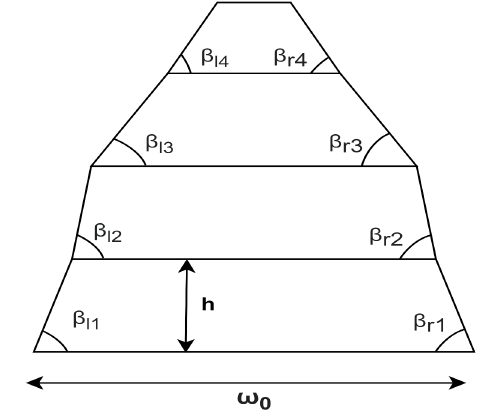
\includegraphics[width=0.3\textwidth]{images/trapezoid.png}
    \caption{Cross-section of a nanostructure line represented as a stack of trapezoids.}
    
\end{figure}
We can calculate the analytical fourier transform of a trapezoidal shape to use for fitting
can be calculated is given by expression:
\begin{equation}
    F\left(q_{x}, q_{z}\right)=\frac{1}{q_{x}}\left[-\frac{m_{1}}{t_{1}} e^{-i q_{x}\left(\frac{\omega_{0}}{2}\right)}\left(1-e^{-i h\left(\frac{q_{x}}{m_{1}}+q_{z}\right)}\right)\right. \\ +\frac{m_{2}}{t_{2}} e^{-i q_{x}\left(\frac{\omega_{0}}{2}\right)}\left(1-e^{\left.-i h\left(\frac{q_{x}}{m_{2}}+q_{z}\right)\right)}\right]
\end{equation}
where,

\( \begin{array}{l}\mathrm{m}_{1}=\tan \left(\beta_{1}\right) m_{2}=\tan \left(\pi-\beta_{r}\right) \\ t_{1}-q_{x}+m_{1} q_{z}\end{array} \)

\medskip

so,
\begin{equation}
    I_{0}(\mathbf{q}) = |F(q)|^{2}
\end{equation}

An additional decay of scattered intensity $I(Q_{x})$ is expected beyond that predicted by the trapezoidal model.
This arises from the distribution of periodicities within the sample. This distribution 
can be caused by two factors:
\begin{itemize}
    \item \textbf{Random variations in average line position}: In this case, the line width remains
         constant, but the average position of the lines fluctuates slightly across the 
         sample.
    \item \textbf{Variations in line width}: Here, the line width itself varies, 
        which also affects the periodicity.
\end{itemize}

Both factors indicate a degree of long-range order within the pattern. Additionally, they provide insights into specific types of line edge roughness [these jerome].

To account for this distribution, we introduce an effective Debye-Waller factor, similar to the one used for fluctuations in crystal lattices.

Hence,

\begin{equation}
    I(\mathbf{q}) = I_{0}(\mathbf{q}) \exp(-q^{2}DW^{2} )
\end{equation}

where $DW$ is the Debye-Waller factor.

\subsection{Experimental setup}
\begin{figure}[h]
    \centering
    \begin{subfigure}[b]{0.8\textwidth}
        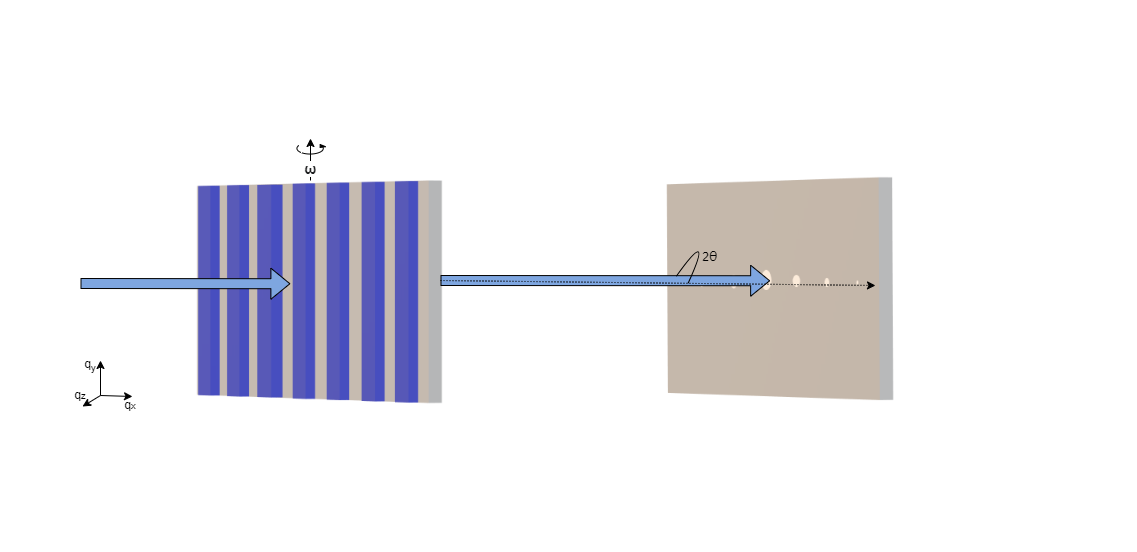
\includegraphics[width=\textwidth]{images/cdsaxs_diff.png}
        \caption{experimental setup}
    \end{subfigure}
    
    \begin{subfigure}[b]{0.4\textwidth}
        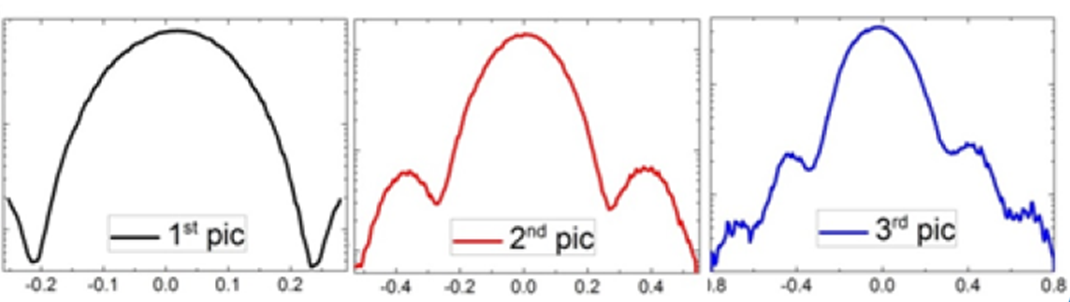
\includegraphics[width=\textwidth]{images/intensity_qz.png}
        \caption{Intensity vs $Q_z$}
    \end{subfigure}
    
    \caption{In a is the schematic of the CD-SAXS instrument layout. The X-ray beam (thick solid lines) is transmitted through the 
    patterned sample. Scattered intensity (I) is measured by a 2D detector as a function of scattering angle $(2\theta)$ 
    and converted to $I(Q_{x})$, where $Q_{x}$ is defined in the text. Measurements are performed at various sample incidence 
    angles $(\theta')$. In b After conversion from the $(Q_{x},\omega)$
    plane, the intensities
   from a trapezoidal cross section would appear as predicted in
   the model calculation on b, plotted as I as a function of the
   Fourier component, $Q_{Z}$.}
   \label{fig:isolated_line}
\end{figure}

\subsection{Fitting Algorithm}

While CDSAXS excels at detecting deviations from a perfect grating pattern in buried structures, it requires additional processing to convert the raw data into a meaningful real-world structure. This process involves using an inverse algorithm, which essentially translates the scattered intensity information back into the original structure's characteristics.

\medskip

However, there's a catch. Traditional optimization methods used for refinement often fall short when dealing with complex internal structures with numerous parameters. These methods rely on iteratively simulating scattering data and comparing it to the measured data. Unfortunately, this approach can be very time-consuming, especially for intricate structures.

\medskip

Another challenge arises from the possibility of "degenerate" solutions. These occur when multiple structural models can produce the same scattering data, making it difficult to pinpoint the true structure. This is a common issue in scattering analysis.

\medskip

Therefore, the ideal scenario for CDSAXS analysis involves an optimization algorithm that can consistently and rapidly converge on the best possible fit for the data. While some prior knowledge about the underlying structure can accelerate the process, such information isn't always readily available. This highlights the need for more efficient algorithms that can handle complex structures even with limited prior knowledge.

\medskip

Previous research has explored various algorithms to determine the optimal set of parameters for a model that best fits the measured CDSAXS data. These parameters essentially describe the actual structure of the nanostructure being analyzed.

\medskip

One approach utilizes a Markov chain Monte Carlo (MCMC) algorithm. However, this method requires a good initial guess for the structure's parameters and limitations on their search range. Additionally, it necessitates multiple independent runs to ensure the algorithm converges on the correct solution. While this approach can be effective, the need for tight parameter bounds might overlook potential fabrication errors in the sample.

\medskip

Another strategy involves massive computing resources with parallelization and highly refined grid-based models. This method, known as reverse MCMC, offers greater accuracy but is limited by the availability of such computational power.

\medskip

Genetic and evolutionary algorithms have emerged as promising alternatives. These methods mimic biological evolution, with the model parameters acting as the "genetic code." Starting with randomly generated parameters, these algorithms iteratively refine them through a "mixing strategy" over multiple generations until the optimal set is found. This approach excels at searching large parameter spaces with wide bounds, making it suitable for complex structures.

\subsubsection{Covariance Matrix Adaptation Evolution Strategy (CMAES)}

One such algorithm is the Covariance Matrix Adaptation Evolution Strategy (CMAES). This method is particularly well-suited for high-dimensional optimization problems, making it ideal for complex nanostructure analysis. CMAES operates by maintaining a population of candidate solutions, with each iteration generating new candidates based on the previous generation's performance. By adapting the covariance matrix of the candidate solutions, CMAES can efficiently explore the parameter space and converge on the optimal solution.

\begin{figure}[h]
    \centering
    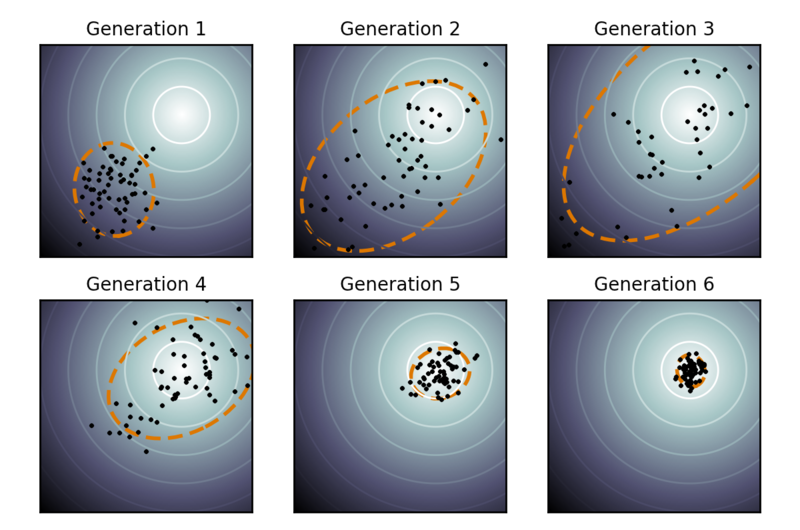
\includegraphics[width=0.8\textwidth]{images/CMAES.png}
    \caption{Illustraion of CMAES algorithm. The algorithm maintains a population of candidate solutions, with each iteration generating new candidates based on the previous generation's performance.(image taken from wikipedia CMAES page) }
    \label{fig:cmaes}
\end{figure}

The code for CD-SAXS generates a set of possible solutions for the parametres of the model. Then we calculate the 
analytical fourier transform of the model and compare it with the experimental data. To compare the two,
we use mean-absolute error log:

\begin{equation}
    \Xi=\frac{1}{N_{\mathrm{q}}-1} \sum_{\overrightarrow{\mathbf{q}}}\left|\log _{10} I_{\mathrm{Sim}}(\overrightarrow{\mathbf{q}})-\log _{10} I(\overrightarrow{\mathbf{q}})\right|
\end{equation}

where $I_{\mathrm{Sim}}(\overrightarrow{\mathbf{q}})$ is the simulated intensity and $I(\overrightarrow{\mathbf{q}})$ is the experimental intensity.

We call it the obtained quantity the goodness of fit. The algorithm then tries to minimize this quantity by adjusting the parameters of the model.

\subsubsection{Uncertainity estimation by Monte Carlo Markov Chain(MCMC) method}


\subsection{Analysis of the reconstructed structure}